%% This is a JAIR Example File Compiled by Nicholas Mattei (nsmattei@tulane.edu) 
%% and Odd Erik Gundersen (odderik@ntnu.no)
%% and Mykel Kochenderfer (mykel@stanford.edu)
%% March 29, 2025
%%
%% This file is based off the ACM Latex Template https://www.acm.org/publications/proceedings-template
%% Revision 2.12 (12/28/2024)
%% 
%% Please see https://www.jair.org/index.php/jair for more information and submission instructions.
%%

%% The first command in your LaTeX source must be the \documentclass
%% command.
%%
%% For submission and review of your manuscript please change the
%% command to \documentclass[manuscript, screen, review]{jair}.
%%
\documentclass[review]{jair}


\setcopyright{cc}
\copyrightyear{2025}
\acmYear{2025}
\acmDOI{10.1613/jair.1.xxxxx}

%%
\JAIRAE{Insert JAIR AE Name}
\JAIRTrack{Insert JAIR Track Name Here}
\acmVolume{4}
\acmArticle{111}
\acmMonth{8}
\acmYear{2025}

%%
%% For managing citations, it is recommended to use bibliography
%% files in BibTeX format.
%%
%% You can then either use BibTeX with the ACM-Reference-Format style,
%% or BibLaTeX with the acmnumeric or acmauthoryear sytles, that include
%% support for advanced citation of software artefact from the
%% biblatex-software package, also separately available on CTAN.
%%
%% Look at the sample-*-biblatex.tex files for templates showcasing
%% the biblatex styles.
%%

%%
%% The majority of ACM publications use numbered citations and
%% references.  The command \citestyle{authoryear} switches to the
%% "author year" style.
%%
%% If you are preparing content for an event
%% sponsored by ACM SIGGRAPH, you must use the "author year" style of
%% citations and references.
%% Uncommenting
%% the next command will enable that style.
%%\citestyle{acmauthoryear}


%%
%% end of the preamble, start of the body of the document source.
\begin{document}

%%
%% The "title" command has an optional parameter,
%% allowing the author to define a "short title" to be used in page headers.
%\title{JAIR Example Template}
\title[Satzilla]{SATzilla: Portfolio-based Algorithm Selection for SAT}

%%
%% The "author" command and its associated commands are used to define
%% the authors and their affiliations.
%% Of note is the shared affiliation of the first two authors, and the
%% "authornote" and "authornotemark" commands
%% used to denote shared contribution to the research and/or corresponding author.
\author{Lin Xu}
\authornote{Corresponding Author.}
\email{xulin730@cs.ubc.ca}
\orcid{0000-0002-2037-3694}
% \orcid{https://orcid.org/0000-0002-2037-3694} % This works too if you want to see the full URL
\affiliation{%
  \institution{University of British Columbia}
  \city{Vancouver}
  \state{British Columbia}
  \country{Canada}
}

\author{Frank Hutter}
\orcid{0000-0002-2037-3694}
\email{hutter@cs.ubc.ca}
\affiliation{%
  \institution{University of British Columbia}
  \city{Vancouver}
  \state{British Columbia}
  \country{Canada}}

\author{Holger H. Hoos}
\orcid{0000-0003-0629-0099}
\email{hoos@cs.ubc.ca}
\affiliation{%
  \institution{University of British Columbia}
  \city{Vancouver}
  \state{British Columbia}
  \country{Canada}
}

\author{Kevin Leyton-Brown}
\orcid{0000-0002-7644-5327}
\email{kevinlb@cs.ubc.ca}
\affiliation{%
  \institution{University of British Columbia}
  \city{Vancouver}
  \state{British Columbia}
  \country{Canada}
}

%\author{Ben Trovato}

%%
%% By default, the full list of authors will be used in the page
%% headers. Often, this list is too long, and will overlap
%% other information printed in the page headers. This command allows
%% the author to define a more concise list
%% of authors' names for this purpose.
\renewcommand{\shortauthors}{Trovato et al.}

%%
%% The abstract is a short summary of the work to be presented in the
%% article.
\begin{abstract}
{\bf Background:} 
    It has been widely observed that there is no single ``dominant'' SAT solver; instead, different solvers perform best on different instances.  
    
    {\bf Objectives:}
    Rather than following the traditional approach of choosing the best solver for a given class of SAT instances, we aim to make this decision fully automatically, online and on a per-instance basis, with the goal of solving a broad range of SAT instances more efficiently in terms of running time. 
    
    {\bf Methods:}
    We describe SATzilla, an automated approach for constructing per-instance algorithm portfolios for SAT that use so-called empirical hardness models to choose among their constituent solvers.  This approach takes as input a distribution of problem instances and a set of component solvers, and constructs a portfolio optimizing a given objective function (such as mean running time, percent of instances solved, or score in a competition).
    In this article, we go well beyond earlier versions of SATzilla, by making the portfolio construction scalable and completely automated, and improving it by integrating local search solvers as candidate solvers, by predicting performance score instead of running time, and by using hierarchical hardness models that take into account different types of SAT instances.  
    
    {\bf Results:}
    The excellent performance of SATzilla was independently verified in the 2007 SAT Competition, where our SATzilla07 solvers won three gold, one silver and one bronze medal. 
    We demonstrate the effectiveness of the new techniques introduced here in extensive experimental results on data sets including instances from the most recent SAT competition.
    
    {\bf Conclusions:}
    The effectiveness of the SATzilla approach demonstrated in this article suggests that per-instance automated algorithm selection may also be possible for NP-hard problems other than SAT. 
    We expect this to pave the way for achieving substantial improvements in the state of the art in solving other important problems in AI and beyond.
\end{abstract}

%\begin{abstract}
%      A clear and well-documented \LaTeX\ document is presented as an
%  article formatted for publication by ACM in a conference proceedings
%  or journal publication. Based on the ``acmart'' document class, this
%  article presents and explains many of the common variations, as well
%  as many of the formatting elements an author may use in the
%  preparation of the documentation of their work.
%\end{abstract}


%% JAIR Note: 
%% Do not include ACM CCS Concepts or Keywords


%% To be updated by authors.
\received{20 February 2007}
\received[revised]{12 March 2009}
\received[accepted]{5 June 2009}

%%
%% This command processes the author and affiliation and title
%% information and builds the first part of the formatted document.
\maketitle

\section{Introduction}
This document describes the revised \LaTeX template used by JAIR starting with volume 83 (2025). The template is based on ACM's consolidated article template, introduced in 2017, which provides a
consistent \LaTeX\ style for use across ACM publications, and
incorporates accessibility and metadata-extraction functionality
necessary for future Digital Library endeavors. JAIR adopted this template because 1) our old template was sadly out of date and we wanted a reliable, maintained template and 2) the journal is now distributed as part of the ACM library (though JAIR remains an independent, open-access journal published by AI Access Foundation, freely available at \url{https://jair.org}). Note that much of the functionality described below relates to ACM publications in general, rather than the specific template used by JAIR.

If you are new to publishing with JAIR or ACM, this document provides a
guide to the process of preparing your work for publication. If you
have published with ACM before, this document provides insight and
instruction into more recent changes to the article template.

The ``\verb|acmart|'' document class can be used to prepare articles
for any ACM publication --- conference or journal, and for any stage
of publication, from review to final ``camera-ready'' copy, to the
author's own version, with {\itshape very} few changes to the source.

\section{Template Overview}
As noted in the introduction, the ``\verb|acmart|'' document class can
be used to prepare many different kinds of documentation --- a
double-anonymous initial submission of a full-length technical paper, a
two-page SIGGRAPH Emerging Technologies abstract, a ``camera-ready''
journal article, a SIGCHI Extended Abstract, and more --- all by
selecting the appropriate {\itshape template style} and {\itshape
  template parameters}.

This document will explain the major features of the document
class. For further information, the {\itshape \LaTeX\ User's Guide} is
available from
\url{https://www.acm.org/publications/proceedings-template}.

There are a number of {\itshape template parameters}
that modify some part of the applied template style. A complete list
of these parameters can be found in the {\itshape \LaTeX\ User's Guide.}

Frequently-used parameters, or combinations of parameters, include:
\begin{itemize}
\item {\texttt{anonymous,review}}: Suitable for a ``double-anonymous''
  conference submission. Anonymizes the work and includes line
  numbers. Use with the \texttt{\acmSubmissionID} command to print the
  submission's unique ID on each page of the work.
\item{\texttt{authorversion}}: Produces a version of the work suitable
  for posting by the author.
\item{\texttt{screen}}: Produces colored hyperlinks.
\end{itemize}

This document uses the following string as the first command in the
source file:
\begin{verbatim}
\documentclass[review]{jair}
\end{verbatim}

\section{Modifications}

Modifying the template --- including but not limited to: adjusting
margins, typeface sizes, line spacing, paragraph and list definitions,
and the use of the \verb|\vspace| command to manually adjust the
vertical spacing between elements of your work --- is not allowed.

{\bfseries Your document will be returned to you for revision if
  modifications are discovered.}

\section{Typefaces}

The ``\verb|acmart|'' document class requires the use of the
``Libertine'' typeface family. Your \TeX\ installation should include
this set of packages. Please do not substitute other typefaces. The
``\verb|lmodern|'' and ``\verb|ltimes|'' packages should not be used,
as they will override the built-in typeface families.

\section{Title Information}

The title of your work should use capital letters appropriately -
\url{https://capitalizemytitle.com/} has useful rules for
capitalization. Use the {\verb|title|} command to define the title of
your work. If your work has a subtitle, define it with the
{\verb|subtitle|} command.  Do not insert line breaks in your title.

If your title is lengthy, you must define a short version to be used
in the page headers, to prevent overlapping text. The \verb|title|
command has a ``short title'' parameter:
\begin{verbatim}
  \title[short title]{full title}
\end{verbatim}

\section{Authors and Affiliations}

Each author must be defined separately for accurate metadata
identification.  As an exception, multiple authors may share one
affiliation. Authors' names should not be abbreviated; use full first
names wherever possible. Include authors' e-mail addresses whenever
possible.

Grouping authors' names or e-mail addresses, or providing an ``e-mail
alias,'' as shown below, is not acceptable:
\begin{verbatim}
  \author{Brooke Aster, David Mehldau}
  \email{dave,judy,steve@university.edu}
  \email{firstname.lastname@phillips.org}
\end{verbatim}

The \verb|authornote| and \verb|authornotemark| commands allow a note
to apply to multiple authors --- for example, if the first two authors
of an article contributed equally to the work.

If your author list is lengthy, you must define a shortened version of
the list of authors to be used in the page headers, to prevent
overlapping text. The following command should be placed just after
the last \verb|\author{}| definition:
\begin{verbatim}
  \renewcommand{\shortauthors}{McCartney, et al.}
\end{verbatim}
Omitting this command will force the use of a concatenated list of all
of the authors' names, which may result in overlapping text in the
page headers.

The article template's documentation, available at
\url{https://www.acm.org/publications/proceedings-template}, has a
complete explanation of these commands and tips for their effective
use.

Note that authors' addresses are mandatory for journal articles.

\section{Rights Information}

JAIR articles are freely available, and a copyright notice referencing the Creative Commons CC BY license is included in the template. This copyright notice should be included in all JAIR articles.

\section{Sectioning Commands}

Your work should use standard \LaTeX\ sectioning commands:
\verb|section|, \verb|subsection|, \verb|subsubsection|, and
\verb|paragraph|. They should be numbered; do not remove the numbering
from the commands.

Simulating a sectioning command by setting the first word or words of
a paragraph in boldface or italicized text is {\bfseries not allowed.}

\section{Tables}

The ``\verb|acmart|'' document class includes the ``\verb|booktabs|''
package --- \url{https://ctan.org/pkg/booktabs} --- for preparing
high-quality tables.

Table captions are placed {\itshape above} the table.

Because tables cannot be split across pages, the best placement for
them is typically the top of the page nearest their initial cite.  To
ensure this proper ``floating'' placement of tables, use the
environment \textbf{table} to enclose the table's contents and the
table caption.  The contents of the table itself must go in the
\textbf{tabular} environment, to be aligned properly in rows and
columns, with the desired horizontal and vertical rules.  Again,
detailed instructions on \textbf{tabular} material are found in the
\textit{\LaTeX\ User's Guide}.

Immediately following this sentence is the point at which
Table~\ref{tab:freq} is included in the input file; compare the
placement of the table here with the table in the printed output of
this document.

\begin{table}
  \caption{Frequency of Special Characters}
  \label{tab:freq}
  \begin{tabular}{ccl}
    \toprule
    Non-English or Math&Frequency&Comments\\
    \midrule
    \O & 1 in 1,000& For Swedish names\\
    $\pi$ & 1 in 5& Common in math\\
    \$ & 4 in 5 & Used in business\\
    $\Psi^2_1$ & 1 in 40,000& Unexplained usage\\
  \bottomrule
\end{tabular}
\end{table}

To set a wider table, which takes up the whole width of the page's
live area, use the environment \textbf{table*} to enclose the table's
contents and the table caption.  As with a single-column table, this
wide table will ``float'' to a location deemed more
desirable. Immediately following this sentence is the point at which
Table~\ref{tab:commands} is included in the input file; again, it is
instructive to compare the placement of the table here with the table
in the printed output of this document.

\begin{table*}
  \caption{Some Typical Commands}
  \label{tab:commands}
  \begin{tabular}{ccl}
    \toprule
    Command &A Number & Comments\\
    \midrule
    \texttt{{\char'134}author} & 100& Author \\
    \texttt{{\char'134}table}& 300 & For tables\\
    \texttt{{\char'134}table*}& 400& For wider tables\\
    \bottomrule
  \end{tabular}
\end{table*}

Always use midrule to separate table header rows from data rows, and
use it only for this purpose. This enables assistive technologies to
recognise table headers and support their users in navigating tables
more easily.

\section{Math Equations}
You may want to display math equations in three distinct styles:
inline, numbered or non-numbered display.  Each of the three are
discussed in the next sections. We note that JAIR authors are discouraged from using sophisticated mathematical notation in the abstract (especially notation that is difficult to reproduce in vanilla HTML), since the abstract will also be formatted in HTML on the JAIR web site. 

\subsection{Inline (In-text) Equations}
A formula that appears in the running text is called an inline or
in-text formula.  It is produced by the \textbf{math} environment,
which can be invoked with the usual
\texttt{{\char'134}begin\,\ldots{\char'134}end} construction or with
the short form \texttt{\$\,\ldots\$}. You can use any of the symbols
and structures, from $\alpha$ to $\omega$, available in
\LaTeX~\cite{Lamport:LaTeX}; this section will simply show a few
examples of in-text equations in context. Notice how this equation:
\begin{math}
  \lim_{n\rightarrow \infty}x=0
\end{math},
set here in in-line math style, looks slightly different when
set in display style.  (See next section).

\subsection{Display Equations}
A numbered display equation---one set off by vertical space from the
text and centered horizontally---is produced by the \textbf{equation}
environment. An unnumbered display equation is produced by the
\textbf{displaymath} environment.

Again, in either environment, you can use any of the symbols and
structures available in \LaTeX\@; this section will just give a couple
of examples of display equations in context.  First, consider the
equation, shown as an inline equation above:
\begin{equation}
  \lim_{n\rightarrow \infty}x=0
\end{equation}
Notice how it is formatted somewhat differently in
the \textbf{displaymath}
environment.  Now, we'll enter an unnumbered equation:
\begin{displaymath}
  \sum_{i=0}^{\infty} x + 1
\end{displaymath}
and follow it with another numbered equation:
\begin{equation}
  \sum_{i=0}^{\infty}x_i=\int_{0}^{\pi+2} f
\end{equation}
just to demonstrate \LaTeX's able handling of numbering.

\section{Figures}

The ``\verb|figure|'' environment should be used for figures. One or
more images can be placed within a figure. If your figure contains
third-party material, you must clearly identify it as such, as shown
in the example below.
\begin{figure}[h]
  \centering
  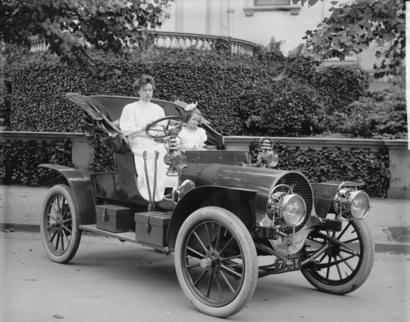
\includegraphics[width=\linewidth]{sample-franklin}
  \caption{1907 Franklin Model D roadster. Photograph by Harris \&
    Ewing, Inc. [Public domain], via Wikimedia
    Commons. (\url{https://goo.gl/VLCRBB}).}
  \Description{A woman and a girl in white dresses sit in an open car.}
\end{figure}

Your figures should contain a caption which describes the figure to
the reader.

Figure captions are placed {\itshape below} the figure.

Every figure should also have a figure description unless it is purely
decorative. These descriptions convey what’s in the image to someone
who cannot see it. They are also used by search engine crawlers for
indexing images, and when images cannot be loaded.

A figure description must be unformatted plain text less than 2000
characters long (including spaces).  {\bfseries Figure descriptions
  should not repeat the figure caption – their purpose is to capture
  important information that is not already provided in the caption or
  the main text of the paper.} For figures that convey important and
complex new information, a short text description may not be
adequate. More complex alternative descriptions can be placed in an
appendix and referenced in a short figure description. For example,
provide a data table capturing the information in a bar chart, or a
structured list representing a graph.  For additional information
regarding how best to write figure descriptions and why doing this is
so important, please see
\url{https://www.acm.org/publications/taps/describing-figures/}.

\section{Citations and Bibliographies}

The use of \BibTeX\ for the preparation and formatting of one's
references is strongly recommended. Authors' names should be complete
--- use full first names (``Donald E. Knuth'') not initials
(``D. E. Knuth'') --- and the salient identifying features of a
reference should be included: title, year, volume, number, pages,
article DOI, etc. 

For managing citations, it is recommended to use bibliography files in BibTeX format.
You can then either use BibTeX with the ACM-Reference-Format style,
or BibLaTeX with the acmnumeric or acmauthoryear styles, that include
support for advanced citation of software artifact from the
biblatex-software package, also separately available on CTAN.

The bibliography is included in your source document with these two
commands, placed just before the \verb|\end{document}| command:
\begin{verbatim}
  \bibliographystyle{ACM-Reference-Format}
  \bibliography{bibfile}
\end{verbatim}
where ``\verb|bibfile|'' is the name, without the ``\verb|.bib|''
suffix, of the \BibTeX\ file.


  Some examples.  A paginated journal article \cite{Abril07}, an
  enumerated journal article \cite{Cohen07}, a reference to an entire
  issue \cite{JCohen96}, a monograph (whole book) \cite{Kosiur01}, a
  monograph/whole book in a series (see 2a in spec. document)
  \cite{Harel79}, a divisible-book such as an anthology or compilation
  \cite{Editor00} followed by the same example, however we only output
  the series if the volume number is given \cite{Editor00a} (so
  Editor00a's series should NOT be present since it has no vol. no.),
  a chapter in a divisible book \cite{Spector90}, a chapter in a
  divisible book in a series \cite{Douglass98}, a multi-volume work as
  book \cite{Knuth97}, a couple of articles in a proceedings (of a
  conference, symposium, workshop for example) (paginated proceedings
  article) \cite{Andler79, Hagerup1993}, a proceedings article with
  all possible elements \cite{Smith10}, an example of an enumerated
  proceedings article \cite{VanGundy07}, an informally published work
  \cite{Harel78}, a couple of preprints \cite{Bornmann2019,
    AnzarootPBM14}, a doctoral dissertation \cite{Clarkson85}, a
  master's thesis: \cite{anisi03}, an online document / world wide web
  resource \cite{Thornburg01, Ablamowicz07, Poker06}, a video game
  (Case 1) \cite{Obama08} and (Case 2) \cite{Novak03} and \cite{Lee05}
  and (Case 3) a patent \cite{JoeScientist001}, work accepted for
  publication \cite{rous08}, 'YYYYb'-test for prolific author
  \cite{SaeediMEJ10} and \cite{SaeediJETC10}. Other cites might
  contain 'duplicate' DOI and URLs (some SIAM articles)
  \cite{Kirschmer:2010:AEI:1958016.1958018}. Boris / Barbara Beeton:
  multi-volume works as books \cite{MR781536} and \cite{MR781537}. A
  couple of citations with DOIs:
  \cite{2004:ITE:1009386.1010128,Kirschmer:2010:AEI:1958016.1958018}. Online
  citations: \cite{TUGInstmem, Thornburg01, CTANacmart}.
  Artifacts: \cite{R} and \cite{UMassCitations}.

\section{Acknowledgments}

Identification of funding sources and other support, and thanks to
individuals and groups that assisted in the research and the
preparation of the work should be included in an acknowledgment
section, which is placed just before the reference section in your
document.

This section has a special environment:
\begin{verbatim}
  \begin{acks}
  ...
  \end{acks}
\end{verbatim}
so that the information contained therein can be more easily collected
during the article metadata extraction phase, and to ensure
consistency in the spelling of the section heading.

Authors should not prepare this section as a numbered or unnumbered {\verb|\section|}; please use the ``{\verb|acks|}'' environment.

\section{Appendices}

If your work needs an appendix, add it before the
``\verb|\end{document}|'' command at the conclusion of your source
document.

Start the appendix with the ``\verb|appendix|'' command:
\begin{verbatim}
  \appendix
\end{verbatim}
and note that in the appendix, sections are lettered, not
numbered. This document has two appendices, demonstrating the section
and subsection identification method.


%%
%% The acknowledgments section is defined using the "acks" environment
%% (and NOT an unnumbered section). This ensures the proper
%% identification of the section in the article metadata, and the
%% consistent spelling of the heading.
\begin{acks}
To Robert, for the bagels and explaining CMYK and color spaces.
\end{acks}

%%
%% The next two lines define the bibliography style to be used, and
%% the bibliography file.
\bibliographystyle{ACM-Reference-Format}
\bibliography{sample-base}


%%
%% If your work has an appendix, this is the place to put it.
\appendix


\section{Research Methods}

\subsection{Part One}

Lorem ipsum dolor sit amet, consectetur adipiscing elit. Morbi
malesuada, quam in pulvinar varius, metus nunc fermentum urna, id
sollicitudin purus odio sit amet enim. Aliquam ullamcorper eu ipsum
vel mollis. Curabitur quis dictum nisl. Phasellus vel semper risus, et
lacinia dolor. Integer ultricies commodo sem nec semper.

\subsection{Part Two}

Etiam commodo feugiat nisl pulvinar pellentesque. Etiam auctor sodales
ligula, non varius nibh pulvinar semper. Suspendisse nec lectus non
ipsum convallis congue hendrerit vitae sapien. Donec at laoreet
eros. Vivamus non purus placerat, scelerisque diam eu, cursus
ante. Etiam aliquam tortor auctor efficitur mattis.

\section{Online Resources}

Nam id fermentum dui. Suspendisse sagittis tortor a nulla mollis, in
pulvinar ex pretium. Sed interdum orci quis metus euismod, et sagittis
enim maximus. Vestibulum gravida massa ut felis suscipit
congue. Quisque mattis elit a risus ultrices commodo venenatis eget
dui. Etiam sagittis eleifend elementum.

Nam interdum magna at lectus dignissim, ac dignissim lorem
rhoncus. Maecenas eu arcu ac neque placerat aliquam. Nunc pulvinar
massa et mattis lacinia.

\section{Reproducibility Checklist for JAIR}

Select the answers that apply to your research -- one per item. 

\subsection*{All articles:}

%\hh{revised for stylistic consistency:}
\begin{enumerate}
    \item All claims investigated in this work are clearly stated. 
    [yes/partially/no]
    \item Clear explanations are given how the work reported substantiates the claims. 
    [yes/partially/no]
    \item Limitations or technical assumptions are stated clearly and explicitly. 
    [yes/partially/no]
    \item Conceptual outlines and/or pseudo-code descriptions of the AI methods introduced in this work are provided, and important implementation details are discussed. 
    [yes/partially/no/NA]
    \item 
    Motivation is provided for all design choices, including algorithms, implementation choices, parameters, data sets and experimental protocols beyond metrics.
    [yes/partially/no]
\end{enumerate}

\subsection*{Articles containing theoretical contributions:}
Does this paper make theoretical contributions? 
[yes/no] 

If yes, please complete the list below.

\begin{enumerate}
    \item All assumptions and restrictions are stated clearly and formally. 
    [yes/partially/no]
    \item All novel claims are stated formally (e.g., in theorem statements). 
    [yes/partially/no]
    \item Proofs of all non-trivial claims are provided in sufficient detail to permit verification by readers with a reasonable degree of expertise (e.g., that expected from a PhD candidate in the same area of AI). [yes/partially/no]
    \item
    Complex formalism, such as definitions or proofs, is motivated and explained clearly.
%hh: was:
%Proof sketches or intuitions are given for complex and/or novel results.
    [yes/partially/no]
    \item 
    The use of mathematical notation and formalism serves the purpose of enhancing clarity and precision; gratuitous use of mathematical formalism (i.e., use that does not enhance clarity or precision) is avoided.
    [yes/partially/no]
    \item 
    Appropriate citations are given for all non-trivial theoretical tools and techniques. 
    [yes/partially/no]
\end{enumerate}

\subsection*{Articles reporting on computational experiments:}
Does this paper include computational experiments? [yes/no]

If yes, please complete the list below.
\begin{enumerate}
    \item 
    All source code required for conducting experiments is included in an online appendix 
    or will be made publicly available upon publication of the paper.
    The online appendix follows best practices for source code readability and documentation as well as for long-term accessibility.
    [yes/partially/no]
    \item The source code comes with a license that
    allows free usage for reproducibility purposes.
    [yes/partially/no]
    \item The source code comes with a license that
    allows free usage for research purposes in general.
    [yes/partially/no]
    \item 
    Raw, unaggregated data from all experiments is included in an online appendix 
    or will be made publicly available upon publication of the paper.
    The online appendix follows best practices for long-term accessibility.
    [yes/partially/no]
    \item The unaggregated data comes with a license that
    allows free usage for reproducibility purposes.
    [yes/partially/no]
    \item The unaggregated data comes with a license that
    allows free usage for research purposes in general.
    [yes/partially/no]
    \item If an algorithm depends on randomness, then the method used for generating random numbers and for setting seeds is described in a way sufficient to allow replication of results. 
    [yes/partially/no/NA]
    \item The execution environment for experiments, the computing infrastructure (hardware and software) used for running them, is described, including GPU/CPU makes and models; amount of memory (cache and RAM); make and version of operating system; names and versions of relevant software libraries and frameworks. 
    [yes/partially/no]
    \item 
    The evaluation metrics used in experiments are clearly explained and their choice is explicitly motivated. 
    [yes/partially/no]
    \item 
    The number of algorithm runs used to compute each result is reported. 
    [yes/no]
    \item 
    Reported results have not been ``cherry-picked'' by silently ignoring unsuccessful or unsatisfactory experiments. 
    [yes/partially/no]
    \item 
    Analysis of results goes beyond single-dimensional summaries of performance (e.g., average, median) to include measures of variation, confidence, or other distributional information. 
    [yes/no]
    \item 
    All (hyper-) parameter settings for 
    the algorithms/methods used in experiments have been reported, along with the rationale or method for determining them. 
    [yes/partially/no/NA]
    \item 
    The number and range of (hyper-) parameter settings explored prior to conducting final experiments have been indicated, along with the effort spent on (hyper-) parameter optimisation. 
    [yes/partially/no/NA]
    \item 
    Appropriately chosen statistical hypothesis tests are used to establish statistical significance
    in the presence of noise effects.
    [yes/partially/no/NA]
\end{enumerate}


\subsection*{Articles using data sets:}
Does this work rely on one or more data sets (possibly obtained from a benchmark generator or similar software artifact)? 
[yes/no]

If yes, please complete the list below.
\begin{enumerate}
    \item 
    All newly introduced data sets 
    are included in an online appendix 
    or will be made publicly available upon publication of the paper.
    The online appendix follows best practices for long-term accessibility with a license
    that allows free usage for research purposes.
    [yes/partially/no/NA]
    \item The newly introduced data set comes with a license that
    allows free usage for reproducibility purposes.
    [yes/partially/no]
    \item The newly introduced data set comes with a license that
    allows free usage for research purposes in general.
    [yes/partially/no]
    \item All data sets drawn from the literature or other public sources (potentially including authors' own previously published work) are accompanied by appropriate citations.
    [yes/no/NA]
    \item All data sets drawn from the existing literature (potentially including authors’ own previously published work) are publicly available. [yes/partially/no/NA]
    %\item All data sets that are not publicly available are described in detail.
    %[yes/partially/no/NA]
    \item All new data sets and data sets that are not publicly available are described in detail, including relevant statistics, the data collection process and annotation process if relevant.
    [yes/partially/no/NA]
    \item 
    All methods used for preprocessing, augmenting, batching or splitting data sets (e.g., in the context of hold-out or cross-validation)
    are described in detail. [yes/partially/no/NA]
\end{enumerate}

\subsection*{Explanations on any of the answers above (optional):}

[Text here; please keep this brief.]

\end{document}
\endinput
%%
%% End of file `sample-acmlarge.tex'.
